\section{Results and discussion}
Experimental results from harvesters are presented in this chapter. Harvesters are tested with various loads and frequencies, 

\subsection{Experimental results of electromagnetic harvester}
This section presents the experimental results from electromagnetic harvester on vibration shaker, both on resistive load and while supplying a harvester board. 

The harvester was built to design presented in \ref{sect:emh_design}. Figure \ref{fig:emh_final} shows the completed assembly. Magnet can be seen suspended in the middle, coil is formed on the upper half of generator. Magnetic spring is formed by magnets on top and bottom sides of the harvester. 

\begin{figure}[htb]
\begin{center}
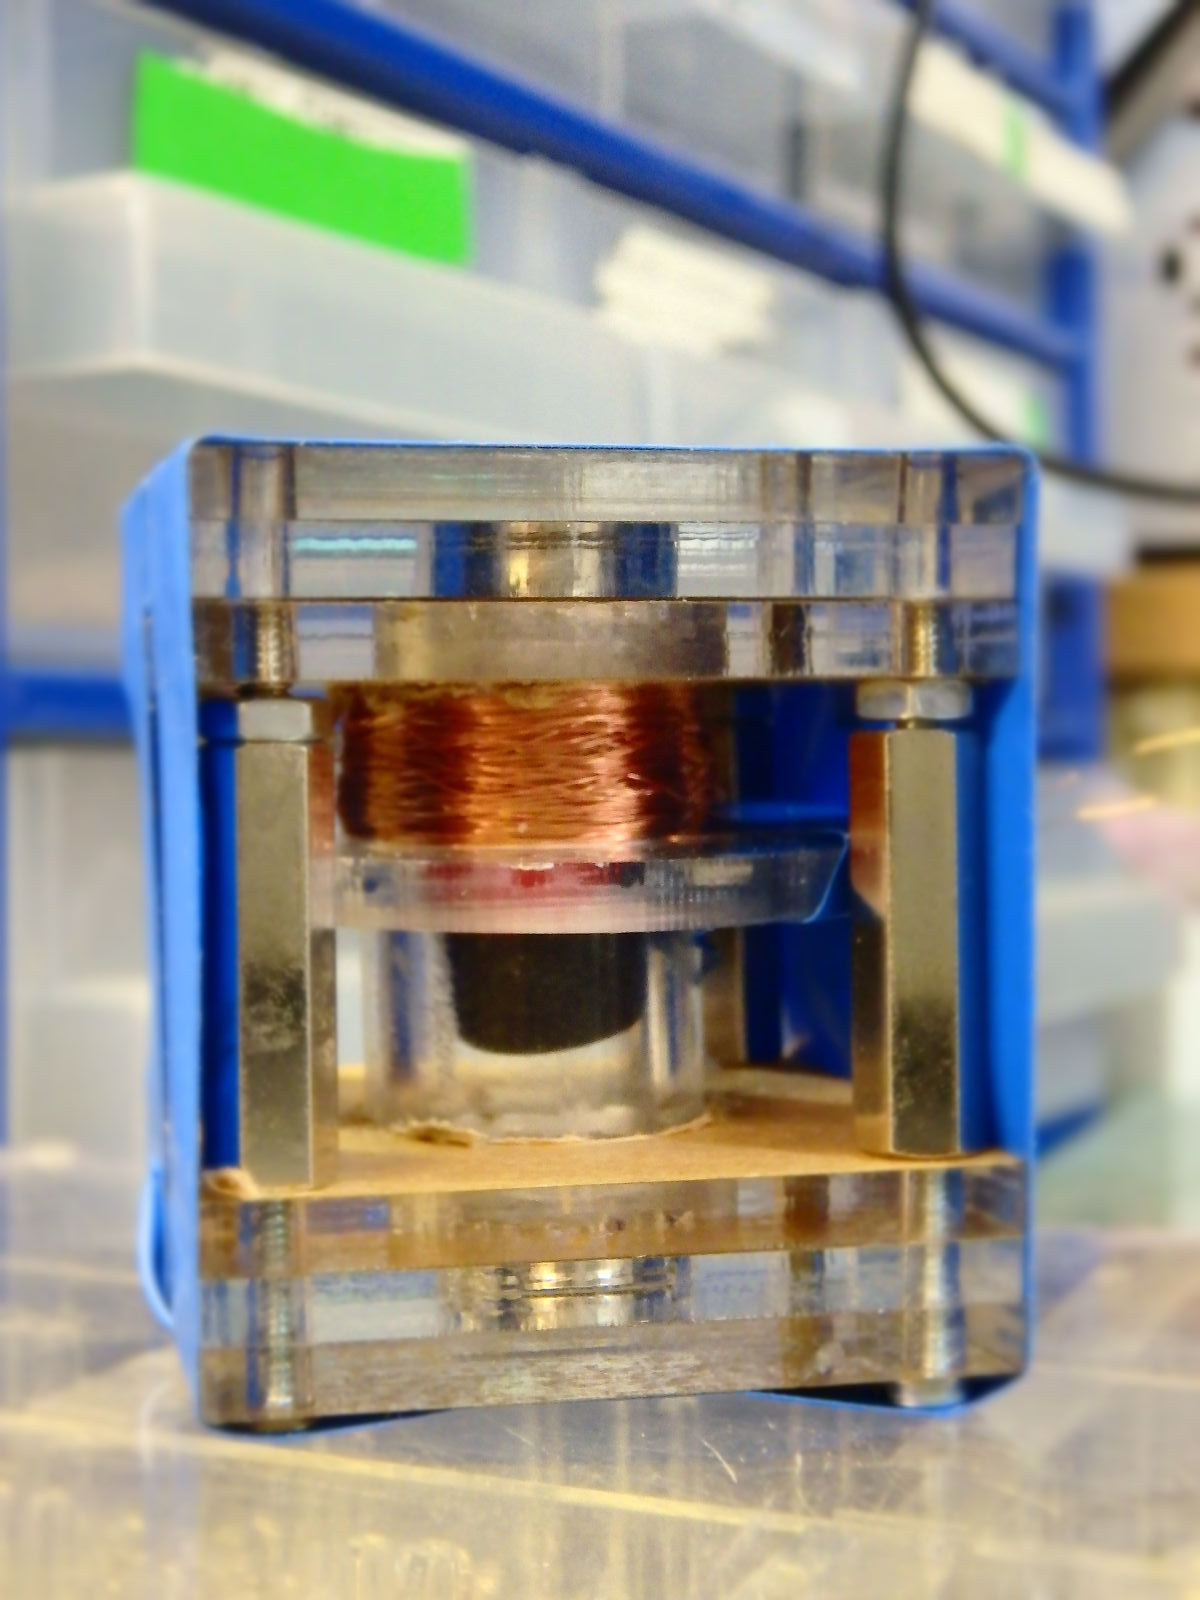
\includegraphics[height=8cm]{images/own_pic/inductive_harvester.jpg}
\end{center}
\caption{\label{fig:emh_final} Finalized electromagnetic harvester.}
\end{figure}


\subsubsection{Test setup} \label{sect:lg_test_setup}
This section details the test setup on vibration exciter. The electromagnetic harvester was connected to vibration exciter Brüel \& Kjær type 4905 for measuring the frequency responce and output power obtainable from the harvester. Figure \ref{fig:emh_shaker} shows the test setup. Syscomp CircuitGear CGR201 oscilloscope was used to generate test signal and take the measurements from harvester. Signal from function generator was amplified by Brüel \& Kjær power amplifier type 2707.

\begin{figure}[htb]
\begin{center}
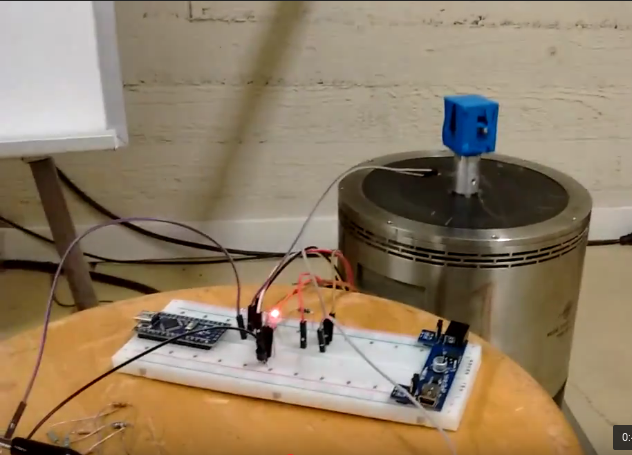
\includegraphics[height=8cm]{images/own_pic/shaker_setup/emh_shaker.png}
\end{center}
\caption{\label{fig:emh_shaker} Test setup for harvester.}
\end{figure}

Regrettably the test setup did not have feedback for position of harvester, so exact displacement or acceleration of harvester is unknown. The output signal from function generator had amplitude of 6 volts peak-to-peak and the gain of power amplifier was set to 9.5 in initial testing, later the function generator amplitude was limited to 2 volts as the response was found to be identical on both settings.

\subsubsection{Time domain results of electromagnetic harvester}\label{sect:lg_td}
First test on the electromagnetic harvester was to measure the timedomain waveforms on various loads and frequencies. After the open loop results were obtained the tests were run again with different resistive loads to measure the power output. Finally the power output to rectifier of harvesting circuit of was measured. This section presents the test results. 

The magnet inside harvester had a notable amount of friction which had to be overcome before any output could be obtained from harvester. It was not possible to obtain very small signals from harvester, as any input strong enough to move the magnet resulted in volt-scale output. Figure \ref{fig:inductive_65_open_dry} shows an example of waveforms obtained from harvester. 

\begin{figure}[htb]
\begin{center}
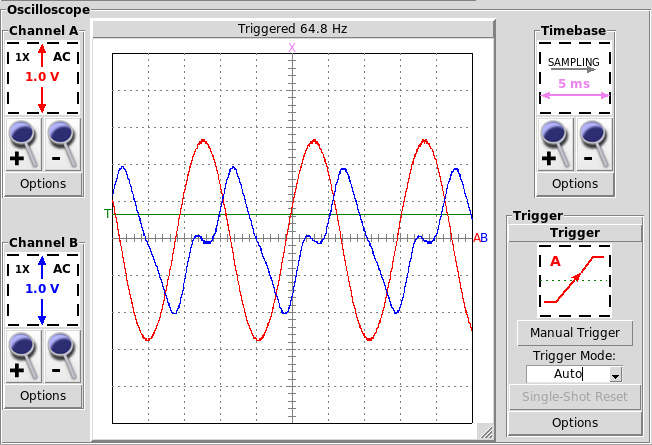
\includegraphics[height=10cm]{images/own_measurement/generator_shaker/inductive_td_open_65hz_dry.png}
\end{center}
\caption{\label{fig:inductive_65_open_dry} Open circuit responce of harvester. Red is excitation waveform, blue is open-circuit voltage from harvester.}
\end{figure}

The waveforms presented in \ref{fig:inductive_65_open_dry} have some curious features: the responce from harvester is asymmetric, there is a notable valley of no output on the rising edge of the signal while no such edge is visible on falling edge. It should be noted that these valleys do not necessarily correspond to direction of gravity: the phase of input/output signal can be inversed at any point in the signal chain as the polarity of magnet, direction of winding of coils, and connection of wires can change.

There seems to be 90 \degree phase shift between excitation and responce. This phase shift was expected, as the excitation signal drives acceleration to shaker, so speed of magnet reaches maximum at zero-crossings of excitation. This observation matches well theory presented in section \ref{sect:em_harvest}: Voltage is proportional to rate of change of magnetic field. 

Amplitude of output is 2 volts and resistance of the coil was measured to be 34 ohms at DC. Inductive component of coil impedance is negligble at the frequencies of interest, so only resistive component needs to be considered. Optimal load would then be 34 ohms. When these values are substituted in time domain into equation \ref{eq:generator_load_power} in section \ref{sect:em_harvest} we obtain

\begin{equation}
\begin{split}
  P_{load}(t)& = V(t) * \frac{ 34 \Omega }{ 34 \Omega + 34 \Omega } * \frac{ V(t) }{ 34 \Omega + 34 \Omega } \\
  P_{load}(t)& = \frac{V(t)^2}{136 \Omega}
\end{split}
\end{equation}

Peak power would be $ \approx 30 mW $. Root mean square (RMS) voltage cannot be accurately calculated from given values, as the waveform is not a perfect sine or triangle wave. If the waveform is approximated as triangle wave, the RMS power would be 

\begin{equation} \label{eq:rms_power}
\begin{split}
  P_{rms}& = k * P_{peak} \\
  P_{rms}& = \frac{1}{\sqrt{3}} * P_{peak} \\
  P_{rms}& \approx 17 mW 
\end{split}
\end{equation}

where $k$ is a constant multiplier for RMS power for triangle waves. 
If the excitation power was increased until rotor magnet audibly contacted the endstop magnets, there was no significant change in output voltage. One possible explanation is the valley in output waveform: maybe the magnet was driven to near-contact to magnet and when the acceleration was reduced the magnet was accelerated by mainly by magnetic interaction. The end result would be that the length of the valley in output waveform would vary while the output amplitude would be limited by magnetic interaction. While further exploration of this phenomenom would be interesting, the testing would be potentially destructive and therefore the tests were left to future work.

Regrettably this harvester cannot be used with the circuit designed in section \ref{sect:electronic_design} as the output amplitude is only 2 volts at any reasonable acceleration and frequency. The circuit would require minimum of 4 volts to get out of undervoltage lockout, and this is not achievable even by connecting the bridge rectifier as voltage doubler as the energy harvesting input still has two diode drops which would keep the voltage below required treshold

Next test was done by connecting the harvester to a boost circuit based on TI BQ25504 \cite{BQ25504}. BQ25504 has a boost-mode SMPS in energy harvesting input which is able to utilise input voltages down to 80 mV after startup and it can start up at roughly 330 mV. The detailed description of the circuit is given in section \ref{sect:BQ25504_schematic}.

To measure the actual power output, a current-to-voltage converter $\mu$Current \cite{muCurrent} was connected in series to harvester output. Measurement was done at scale $1 V = 1 mA$. Waveforms are shown in figure \ref{fig:inductive_vi_65}. It should be noted that the current channel might be saturated, as $\mu$Current cannot produce output higher than 1.25 V.

\begin{figure}[htb]
\begin{center}
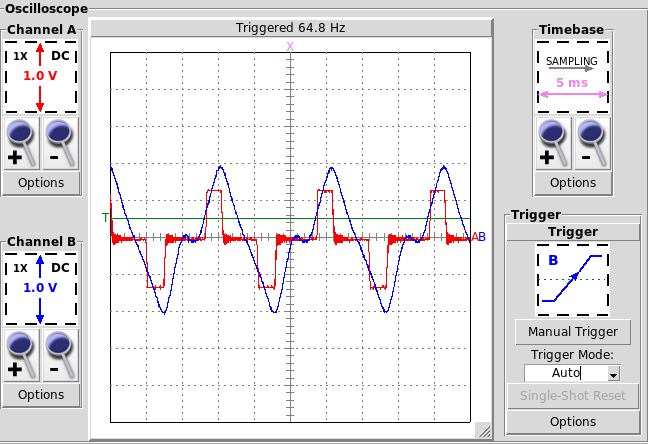
\includegraphics[height=10cm]{images/own_measurement/generator_shaker/inductive_td_harvesting_vi_65hz_ferro.png}
\end{center}
\caption{\label{fig:inductive_vi_65} Voltage and current waveform from harvester. Red is current, 1 V equals 1 mA. Blue is voltage from the terminals of harvester before rectification.}
\end{figure}

The waveforms are as expected, there is no current flowing while voltage is low. When the voltage rises to roughly one volt, current starts to flow charging the output capacitor. When input voltage starts to decrease, no more current flows to capacitor. Accuracy of amplitude of current measurement is questionable because of potential saturation of measuring instrument.

It is worth noting that the voltage rises to open-loop maximum amplitude of 2 V as the loading on harvester decreases as the voltage on capacitor increases. This indicates that maximum theoretical peak power output of $\approx$ 30 mW is not reached at any point. 

Power waveform of harvester is presented in figure \ref{fig:inductive_power_65}. The waveform is calculated by multiplying the voltage and current. Because current is scaled at 1 mA = 1 V, the result can be read as 1 V = 1 mW. While absolute value of power is questionable because of potentially saturated instrument, the waveform itself is correct.  

\begin{figure}[htb]
\begin{center}
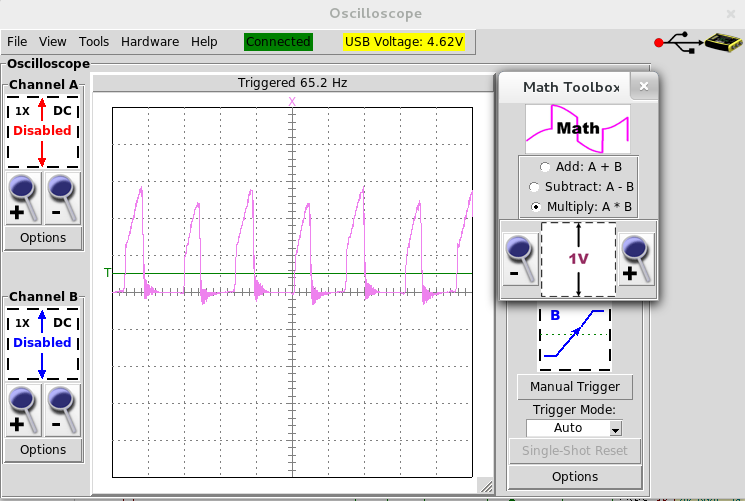
\includegraphics[height=10cm]{images/own_measurement/generator_shaker/inductive_td_harvesting_power_65Hz_ferro.png}
\end{center}
\caption{\label{fig:inductive_power_65} Power waveform from harvester. Pink is power, 1 V equals 1 mW.}
\end{figure}

Graphically read average power output is 0.375 mW. One possible reason for the greatly lesser power output was the capacitors in voltage doubler structure: the voltage doubler has series capacitance of 10 $\mu$F, which has reactive impedance of

\begin{equation}
\begin{split}
  X_c& = \frac{1}{2 \pi f C} \\
  X_c& = \frac{1}{2 \pi 65 10\mu} \\
  X_c& \approx 245 \Omega
\end{split}
\end{equation}

at 65 Hz. Total output impedance of circuit would be approximately 280 $\Omega$, which would limit the output current to approximately 7 mA. This theory was tested by simulating the equivalent model of input section of harvester circuit. Simulation model and results are shown in figure \ref{}

\begin{figure}[htb]
\begin{center}
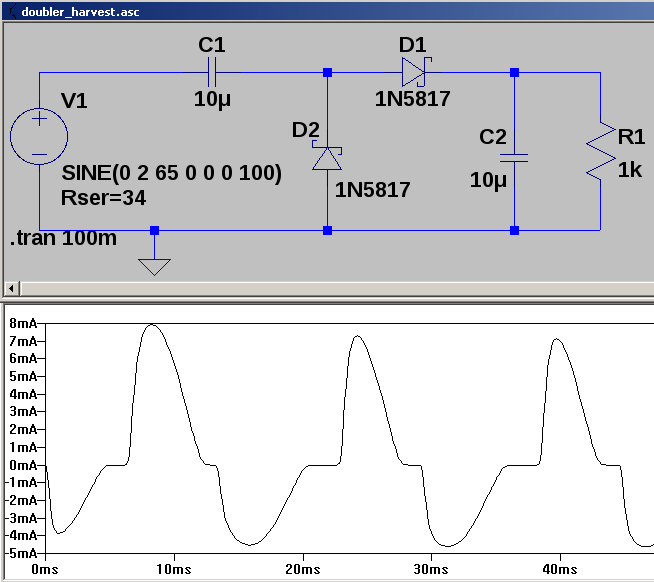
\includegraphics[height=10cm]{images/own_dwg/simulation/voltage_doubler.png}
\end{center}
\caption{\label{fig:simulated_doubler} LTSpice model of energy harvester input section.}
\end{figure}

The simulated data confirms the effect of input capacitor to current output of system. Current is limited to roughly 7 mA. Simulated power output was on average 2.0 mW. If the measured current is assumed to be limited by saturation, and if we assume that simulated current of 8 mA peaks would be correct, the calculated power output from experimental result would be 

\begin{equation}
\begin{split}
  P_{true}& = P_{simulated} * \frac{I_{simulated}}{I_{real}} \\
  P_{true}& = 0.375 * \frac{7}{1.25} \\
  P_{true}& = 2.1 mW. \\
\end{split}
\end{equation}

After correcting the experimental current with simulated value, a lot more reasonable value of approximately 2 mW of generated power is obtained. 

This section presented the time-domain results of the electromagnetic harvester on a shaker test platform. Approximately 30 mW peak power was obtained, RMS power of 17 mW was achieved to resistive load and power output to harvester was determined to be in range between 0.4 mW and 2 mW. Next section presents the frequency domain measurements of the generator as well as studies the effect of application of ferrofluid to harvester.

\subsubsection{Frequency domain results of electromagnetic harvester}
One of the original design goals of the harvester was to provide a wide-band energy harvester solution. This section presents the frequency domain responce of the electromagnetic harvester.

Frequency domain responce was obtained by sweeping a wide-band sine signal to power amplifier and measuring the open loop responce from harvester. The first measurement was done on a harvester without ferroluid applied, figure \ref{fig:inductive_fd_dry} displays the measurement result. Above graph is output in decibels, below is the phase shift of the responce.

\begin{figure}[htb]
\begin{center}
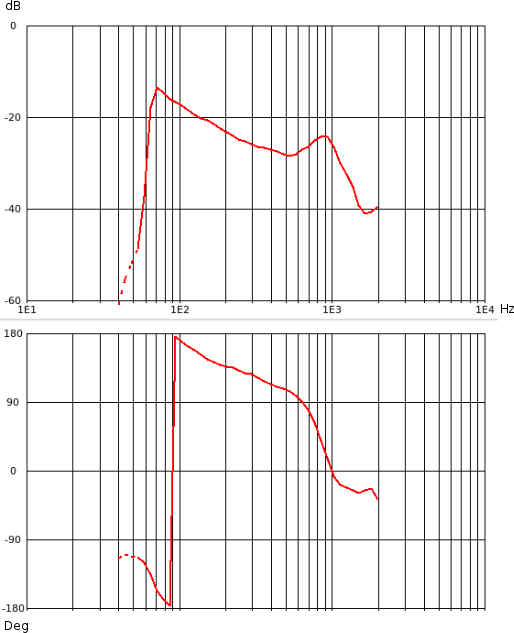
\includegraphics[height=10cm]{images/own_measurement/generator_shaker/inductive_fd_dry.png}
\end{center}
\caption{\label{fig:inductive_fd_dry} Frequency domain responce of electromagnetic harvester before application of ferrofluid.}
\end{figure}

There is a clear resonance peak near 70 Hz. The phase shift is almost exactly 180 \degree at the resonance, which is somewhat curious result as the time domain results and theory predicted the voltage would peak at 90 \degree phase when the acceleration is at zero and speed is at highest. 

Amplitude does not have any specific meaning outside the context of this measurement and comparing output at different frequencies. It can be seen that original design goal of wide band responce has not been achieved very well, as the amplitude responce rolls off sharply below the effective frequency and maybe 20 dB / decade on frequencies above the peak. There is another resonance peak near 900 Hz, but this frequency is far above frequencies of interest for the application. 

Ferrofluid was applied to rotor magnet in attempt to reduce the effect of friction, and bode diagram was similarily plotted to figure \ref{fig:inductive_bode_ferro}.

\begin{figure}[htb]
\begin{center}
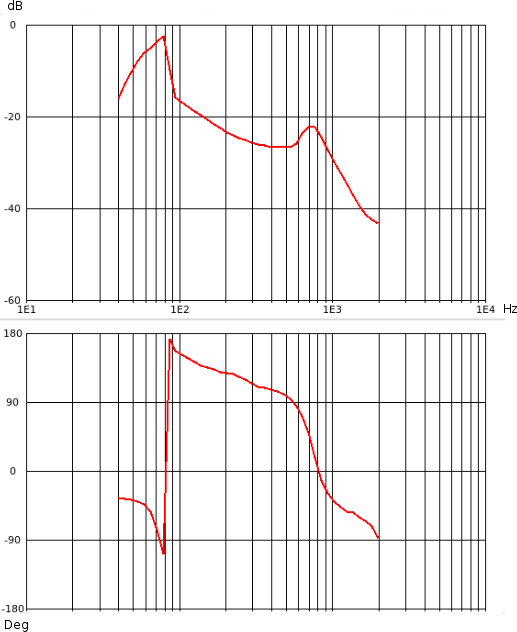
\includegraphics[height=10cm]{images/own_measurement/generator_shaker/inductive_bode_ferro.png}
\end{center}
\caption{\label{fig:inductive_bode_ferro} Frequency domain responce shows a strong resonance peak after application of ferrofluid.}
\end{figure}

The application of ferrofluid shows a strong resonance peak near 70 Hz, phase shift behaviour is similar to non-lubricated experiment. Usually the systems which have second order dynamics - such as the mass damper spring system - exhibit resonance peaks when dampening factor is low. It is therefore obvious that application of ferrofluid has resulted in lesser frictional losses. Amplitude responce is also at higher level across all frequencies, suggesting a better overall performance. 

\subsection{Experimental results of piezoelectric harvester}

\subsubsection{Time domain results of piezoelectric harvester}
This section presents the time-domain results of the piezoelectric harvester. The test setup of piezoelectric harvester was similar to the test setup of electromagnetic harvester, details of the test setup are given in section \ref{sect:lg_test_setup}. Unlike electromagnetic harvester, this piezoelectric harvester did not have any obvious minimum acceleration before friction would be overcome and therefore even very small signal was obtainable. Likewise no maximum value for output signal was found by increasing the power to vibration exciter. The function generator output signal was held at 6 volts peak-to-peak for time domain tests and at 3 volts peak-to-peak for frequency domain tests to limit the loosening of screws by vibration.

The piezoelectric harvester was characterized by high output voltages at high output impedances. Open loop response is shown in figure \ref{fig:piezo_td_open}. The output was not a clean sine-resembling signal as with electromagnetic harvester, it has sharp downwards peaks and a lot of high-frequency distortion.

\begin{figure}[htb]
\begin{center}
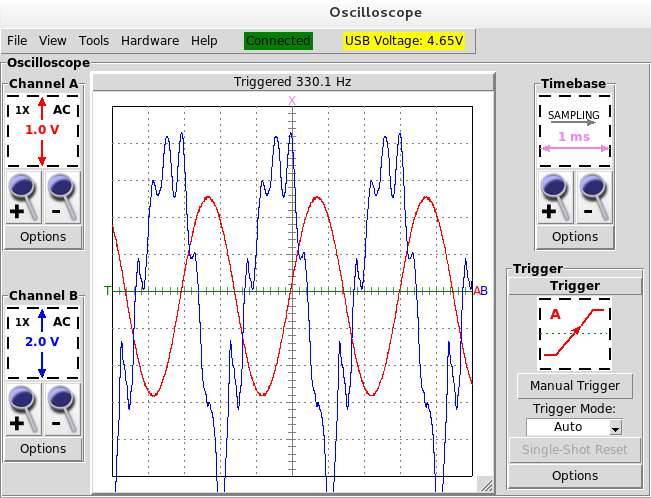
\includegraphics[height=10cm]{images/own_measurement/generator_shaker/piezo_td_open_330hz_2_2.png}
\end{center}
\caption{\label{fig:piezo_td_open} Open loop response from piezoelectric harvester. Red is excitation signal, blue is response.}
\end{figure}

While output signal is off the scale, negative peaks were measured at -12 volts. Peak-to-peak amplitude was therefore roughly 20 volts. The search for maximum power point was started by modeling circuit as RC- high pass filter shown in figure\ref{fig:rc_highpass} with piezo capacitance as the series capacitor and load as the resistor. 

\begin{figure}[htb]
\begin{center}
\includegraphics[height=4cm]{images/cited/hyperphysics.jpg}
\end{center}
\caption{\label{fig:rc_highpass} RC high pass filter \cite{hyperphysics}.}
\end{figure}

The frequency domain results presented in section \ref{sect:piezo_fd} were used to find the maximum output frequency at 330 Hz. This frequency was taken as the target cut-off frequency for the RC-filter equation:

\begin{equation}
\begin{split}
  F_c &= \frac{1}{2 \pi R C} \\
  R   &= \frac{1}{2 \pi C F} \\
  R   &= \frac{1}{2 \pi 39 nF 330 Hz} \\
  R   &\approx 12 400 \Omega 
\end{split}
\end{equation}

Theory would predict the maximum power point to be near the cut-off frequency, so the generator was tested with 18k, 12k and 9k ohm resistive loads. The peak voltages and calculated power into load are presented in table \ref{tbl:piezo_harvester_shaker_output}. The power is calculated by approximating the waveform as a clean sine calculating RMS power from peak voltage values. Method is similar to equation \eqref{eq:rms_power} presented in section \ref{sect:lg_td}, but the multiplier $k$ is $\sqrt{2}$ instead of $\sqrt{3}$ as the waveform is approximated as sine rather than triangle. While the absolute value of power output suffers from approximation error, the waveforms obtained with 18 k$\Omega$ and 12 k$\Omega$ are similar enough for comparing the outputs between loads. On 9 k$\Omega$ load the waveform was clearly more distorted, and therefore the output was notably smaller than calculated.

\begin{table}[htb]
\caption{\label{tbl:piezo_harvester_shaker_output} Output power of piezo harvester at various 18k, 12k and 9k $\Omega$ loads.}
\begin{center}
\fbox{
\begin{tabular}{l l l}
\textbf{Load}          & \textbf{Amplitude} 		& \textbf{Power\textsubscript{rms}}	\\ \hline
18k $\Omega$  & 7 volts	& 1.36 mW 		\\ \hline
12k $\Omega$  & 6 volts	& 1.50 mW	\\ \hline
9k  $\Omega$  & 4 volts 	& 0.89 mW
\end{tabular}
}
\end{center}
\end{table}

The waveforms from 12 k$\Omega$ load and 9 k$\Omega$ load are shown in figures \ref{fig:piezo_td_12k} and \ref{fig:piezo_td_9k} for comparing the amount of distortion. While both waveforms show a clear high-frequency content, possibly caused by resonant frequency of piezo element itself, the heavier loading causes a significant distortion on the waveform.

\begin{figure}[htb]
\begin{center}
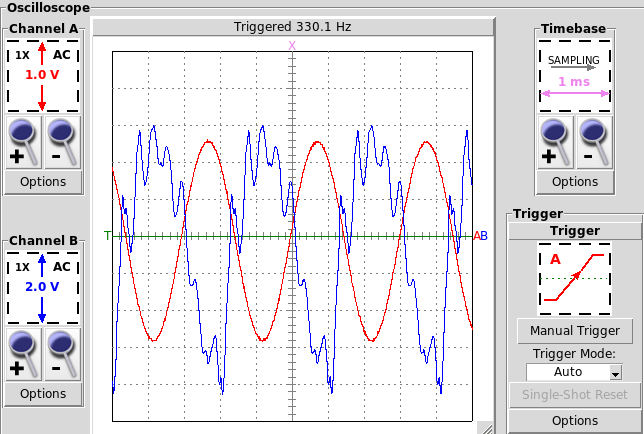
\includegraphics[height=10cm]{images/own_measurement/generator_shaker/piezo_td_12k_330hz_2_2.png}
\end{center}
\caption{\label{fig:piezo_td_12k} Piezoelectric harvester under 12 k$\Omega$ load. Red is excitation signal, blue is response.}
\end{figure}

\begin{figure}[htb]
\begin{center}
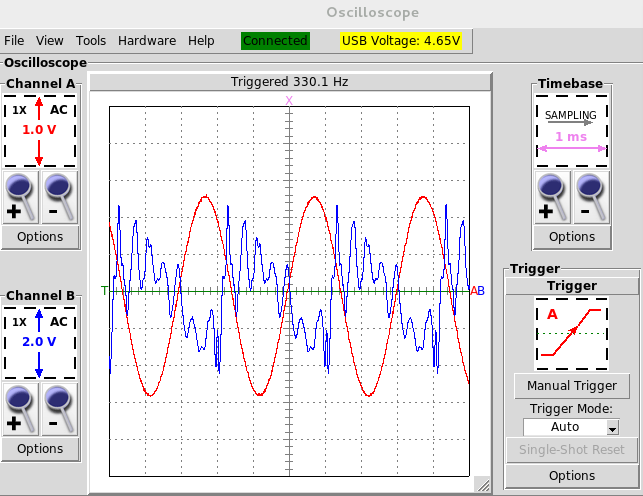
\includegraphics[height=10cm]{images/own_measurement/generator_shaker/piezo_td_9k_330hz_2_2.png}
\end{center}
\caption{\label{fig:piezo_td_9k} Piezoelectric harvester under 9 k$\Omega$ load. Red is excitation signal, blue is response.}
\end{figure}

The waveform on figure \ref{fig:piezo_td_9k} resembles almost a saw-tooth wave. Regardless of actual RMS value, it can be confidently said that the power output is smaller under 9 k$\Omega$ load than under 12 k$\Omega$ load. Therefore maximum power point can be concluded to be near 12 k$\Omega$ load at 330 Hz. 

After testing behaviour on resistive loads, power output to harvester through rectification was tested. While the electromagnetic harvester had notably higher output to resistive load, rectification drops voltage and therefore high-voltage characteristic of piezoelectric harvester is advantageus. 

As with the electromagnetic harvester, current was measured using $\mu$Current at 1 mV / uA setting. While electromagnetic harvester suffered from reactance of series capacitance limiting the output of harvester, output impedance of piezoelectric harvester is a lot higher than that of additional series capacitor and therefore output was not impaired by coupling capacitance. The VI-waveforms are shown in figure \ref{}

\subsection{Harvestering circuit results }
Text on BQ25504 instead of LTC3331, possibly testbench results of LTC3331?

\subsection{Performance inside tyre}
Testing inside tyre, matrix of power outputs. 

